\documentclass{homework}
% \usepackage{graphicx} % Required for inserting images
\usepackage{amsmath}
\usepackage{amsthm}
\usepackage{gensymb}
\usepackage{subfig}
\usepackage{float}

\class{ECEN 5448}
\title{Homework 2}
\author{Sean Jennings}
\date{October 7, 2023}

\begin{document}
\maketitle

\section{Solutions of Linear Differential Equations}
\subsection{Problem 1.1}
\begin{letterenum}
    \item Since $x_1(t)$ and $x_2(t)$ are solutions to the given homogeneous system,
        there exists a unique state transition matrix $\Phi: \R \times \R \to \R^{n \times n}$
        (given by the Peano-Baker Series) such that:
        \begin{equation}
            x_1(t) = \Phi(t, t_0) x_1(t_0) \qquad x_2(t) = \Phi(t, t_0) x_2(t_0)
        \end{equation}
        for all $t_0 \in \R$, $t_0 \geq 0$. Then, given a time $t$ at which $x_1(t) = 2x_2(t)$, it follows that
        \begin{equation}
            \Phi(t, t_0)x_1(t_0) = 2 \Phi(t, t_0)x_2(t_0).
        \end{equation}
        Since the state transition matrix is invertible across its domain,
        it follows that $x_1(t_0) = 2x_2(t_0)$ for all $t_0\geq0$. In particular,
        putting $t_0 = 0$, we find $x_1(0) = 2x_2(0)$,
        but in fact, this relation holds for all of time!

    \item No, as $t\to\infty$, trajectories w/ different initial conditions can all converge
    to the same point. For example,
    \begin{equation}
        \dot{x} = A x \qquad A = \mat{-1 & 0 \\ 0 & -1}
    \end{equation}
    has solution
    \begin{equation}
        x(t) = e^{At}x(0) = \mat{e^{-t} & 0 \\ 0 & e^{-t}} x(0).
    \end{equation}
    Then, $\lim_{t\to\infty}x(t) = 0$ for all $x(0) \in \R^2$. Therefore, we can pick
    any two initial points $x_1(0),x_2(0)\in\R^2$ such that $x_1(0) \neq x_2(0)$
    and $\lim_{t\to\infty}x_1(t) = \lim_{t\to\infty}x_2(t)$, which contradicts
    the proposition in question.
\end{letterenum}

\subsection{Problem 1.2}
\renewcommand{\N}{\mathcal{N}}

\begin{letterenum}
    \item We begin by rearranging terms to rewrite the system in matrix
        form.
        \begin{align*}
            \dot{\theta}_i &= \frac{1}{|\N_i|} \sum_{j \in \N_i} \frac{1}{\alpha(t)}
                (\theta_j - \theta_i) \\
                &= \frac{1}{\alpha(t)}\biggl[
                    \frac{1}{|\N_i|} \sum_{j\in\N_i} (\theta_j) - \theta_i
                \biggr].
        \end{align*}
        Then, $\dot{x} = A(t) x$ where
        \begin{equation}
            A(t) = \frac{1}{\alpha(t)}\mat{
                -1 & 1& 0 \\
                1/2 & -1 & 1/2 \\
                0 & 1 & -1
            }
            \label{eq:a-matrix-birds}
        \end{equation}
        Define $B$ as the time-invariant component of the matrix on the
        right hand side of equation (\ref{eq:a-matrix-birds}) such that
        $A(t) = \frac{1}{\alpha(t)} B$. Since only the scalar component
        $\alpha(t)\in\R$ of $A(t)$ is time-varying, we can verify that $A(t)$
        commutes with its integral $\int_{0}^{t}A(\tau)d\tau$:
        \begin{align*}
            A(t) \int_{0}^{t}A(\tau)d\tau &=
                    \frac{1}{\alpha(t)}B
                    \int_{0}^{t}\frac{1}{\alpha(t)}B d\tau \\
                &= \frac{1}{\alpha(t)}
                    \int_{0}^{t}\frac{1}{\alpha(t)}B^2 d\tau \\
                &= \int_{0}^{t}\frac{1}{\alpha(t)}B d\tau
                    \biggl(\frac{1}{\alpha(t)}B\biggr)\\
                &= \int_{0}^{t} A(\tau)d\tau A(t)
        \end{align*}
        Therefore, we can find an analytic solution to the system (as in the
        case of a 1-dimensional LTV system):
        \begin{align}
            x(t) &= e^{\int_{0}^{t} A(\tau)d\tau} x(0) \\
                &= (e^B)^{\int_{0}^{t} \frac{1}{\alpha(\tau)}d\tau} x(0).
        \end{align}
        We note that since we are given numerical values for the matrix $B$,
        we can compute $e^B$ via its jordan normal (and the sympy Python package):
        \begin{equation}
            B = PJP^{-1}
        \end{equation}
        where
        \begin{equation}
            P = \mat{
                 1 & -1 & 1 \\
                -1 &  0 & 1 \\
                 1 &  1 & 1
            } \qquad J = \mat{
                -2 & 0 & 0 \\
                0  &-1 & 0 \\
                0  & 0 & 0
            } \qquad P^{-1} = \frac{1}{4}\mat{
                1 & -2 & 1 \\
               -2 &  0 & 2 \\
                1 &  2 & 1 \\
            }
        \end{equation}
        which yields the exponential:
        \begin{equation}
            e^B = Pe^J P^{-1} \approx \mat{
                0.468 & 0.432 & 0.0999  \\
                0.216 & 0.568 & 0.216  \\
                0.0999 & 0.432 & 0.468
            }
        \end{equation}
        We note here that any vector $x=[\theta_1, \theta_2, \theta_3]^T$ with
            $\theta_1=\theta_2=\theta_3$ is an equilibrium position and is
            represented by the third column of $P$, with eigenvalue 0,
            therefore remaining constant over time.

    \item For $\alpha(t) = e^t$, we have
    \begin{equation}
        \int_{0}^{t}\frac{1}{e^\tau}d\tau = \int_{0}^{t} e^{-\tau} d\tau
            = -e^{-\tau} \eval_0^t = 1 - e^{-t}
    \end{equation}
    which has limit,
    \begin{equation}
        \lim_{t\to\infty}\int_{0}^{t}\frac{1}{\alpha(t)}d\tau = 1.
    \end{equation}
    Therefore,
    \begin{equation}
        \lim_{t\to\infty}x(t) = (e^B)^1 x(0) = \boxed{e^B x(0)}
    \end{equation}
    We note that since $A(t)$ exponentially decays from $B$ to $0$, the flock
    does not reach their equilibrium position. The decaying components
    corresponding to the first two columns of $P$ (representing the birds'
    relative positions) only decay to $e^{-2}$ and $e^{-1}$, a fraction
    of the distance to the equilibrium position.

    \item For $\alpha(t) = t+1$, we have
    \begin{equation}
        \int_{0}^{t}\frac{1}{\alpha(\tau)}d\tau = \int_{0}^{t}\frac{d\tau}{\tau + 1}
            = \ln{|t+1|}
    \end{equation}
    which gives:
    \begin{align*}
        \int_{0}^{t} A(\tau)d\tau &= B \int_{0}^{t}\frac{1}{\alpha(\tau)} d\tau
            &= P \mat{
                -2\ln|t+1| & 0 & 0 \\
                0  &-\ln|t+1| & 0 \\
                0  & 0 & 0
            } P^{-1}
    \end{align*}
    taking the exponential yields:
    \begin{align*}
        e^{\int_{0}^{t}A(\tau)d\tau} &= P \mat{
            e^{-2\ln|t+1|} & 0 & 0 \\
            0  &e^{-\ln|t+1|} & 0 \\
            0  & 0 & e^0
        } P^{-1} \\
        &= P \mat{
            1/(t+1)^2 & 0 & 0 \\
            0  & 1/|t+1| & 0 \\
            0  & 0 & 1
        } P^{-1}
    \end{align*}
    Now, we compute the limit:
    \begin{align*}
        \lim_{t\to\infty} x(t) &= P \mat{
            0 & 0 & 0 \\
            0 & 0 & 0 \\
            0 & 0 & 1
        } P^{-1} x(0) \\
        &= \frac{1}{4} \mat{
            1 & 2 & 1 \\
            1 & 2 & 1 \\
            1 & 2 & 1
        } x(0)
    \end{align*}
    So, the system approaches a weighed average of its initial position. The
    (exponential) rate at which the system approaches its equilibrium ($\norm{x(t) - x^*}$)
    outstrips the (linear) rate that the magnitude of that response (the matrix $A(t)$)
    decays.

    In terms of birds, the system achieves flocking with the initial direction
    of the second bird having additional greater influence on their final heading.
    A similar interpretation can be reached
    with the change of coordinates $y=P^{-1}x$ (and multiplying both side by
    $P^{-1})$:
    \begin{equation}
        \lim_{t\to\infty}y(t) = \mat{
            0 & 0 & 0 \\
            0 & 0 & 0 \\
            0 & 0 & 1
        } y(0) = \mat{
            0 \\ 0 \\ y_2(0)
        }
    \end{equation}
    
    


\end{letterenum}

\subsection{Problem 1.3}
Using the semigroup property of the state transition transition matrix, we have
\begin{equation}
    \Phi(2,1) = \Phi(2, 0)\Phi(0, 1) = \Phi(2, 0)\Phi(1, 0)^{-1}.
\end{equation}
This easily evaluates using a digital computer to
\begin{align*}
    \Phi(2, 1) &= \mat{
        -4.83 & -0.0139  \\
        5.59 & -0.0120
    } \mat{
        -1.13 & 0.123  \\
        -2.47 & -0.0563
    }^{-1} \\
    &= \mat{
        -4.83 & -0.0139  \\
        5.59 & -0.0120
    } \mat{
        -0.153 & -0.335  \\
        6.72 & -3.07
    } \\
    &= \boxed{\mat{
        0.646 & 1.66  \\
        -0.937 & -1.83
    }}
\end{align*}

\section{Norms on vector spaces}
\subsection{Problem 2.1}
We begin by finding an upper bound on $\normi{A}$. 
For any $x\in\R^n$, by definition of $\norm{\cdot}$,
triangle inequality, and the submultiplicity property, respectively,
we have
\begin{align}
    \normi{Ax} &= \max_i \biggl\{
        \biggl\rvert \sum_{j=1}^{n}  a_{ij}x_j \biggr\rvert
    \biggr\} \\
    &\leq \max_i \biggl\{
        \sum_{j=1}^{n}  | a_{ij}x_j |
    \biggr\} \\
    &\leq \max_i \biggl\{
        \sum_{j=1}^{n}  | a_{ij}||x_j |
    \biggr\}
    \label{eq:ax-bound}
\end{align}
where $i\in[1, 2, \dots, m]$.

By definition of induced matrix norm, we have
\begin{equation}
    \normi{A} = \max_{x\in\R^n} \biggl\{
        \normi{Ax}: \normi{x} = 1
    \biggr\}
    \label{eq:inf-norm}
\end{equation}
so that $|x_j|\leq 1$ for each $j\in[1,2,\dots,n]$. 
Thus, applying the constraints of equation (\ref{eq:inf-norm})
to the upper bound of equation (\ref{eq:ax-bound}) yields
the bound
\begin{equation}
    \normi{A} = \max_i \biggl\{
        \sum_{j=1}^n |a_{ij}|
    \biggr\}
    \label{eq:norm-upper-bound}
\end{equation}
for $i\in[1, 2, \dots,m]$.

It remains to show the upper bound is attained. Select $I\in[1,2,\dots,m]$
to be the index of the row with the maximum sum of absolute values:
\begin{equation}
    I = \text{arg}\max_i \biggl\{\sum_{j=1}^n |a_{ij}|\biggr\}
    \label{eq:index}
\end{equation}

Then select $x_j^*$ s.t.
\begin{equation}
    x_j^* = \biggl\{
        \begin{array}{ll}
            1 &\quad \text{if } a_{Ij} \geq 0 \\
            -1 &\quad \text{otherwise}
        \end{array}
    \biggr.
\end{equation}
It's easy to verify $a_{Ij}x_j^* = |a_{Ij}|$ for all $j$. Then,
we can compute a lower bound for $\normi{Ax^*}$:
\begin{align*}
    \normi{Ax^*} &= \max_i \biggl\{
        \biggl\rvert \sum_{j=1}^n a_{ij}x_j^* \biggr\rvert
    \biggr\}\\
        &\geq \biggl\rvert \sum_{j=1}^n a_{Ij}x_j^* \biggr\rvert \\
        &= \biggl\rvert \sum_{j=1}^n |a_{Ij}| \biggr\rvert \\
        &= \sum_{j=1}^n |a_{Ij}|
\end{align*}
By equations (\ref{eq:norm-upper-bound}) and (\ref{eq:index}),
$\normi{Ax^*}$ is upper bounded by the same expression and thus becomes an equality.
Therefore, the upper bound of $\normi{A}$ is attained by $\normi{Ax^*}$:
\begin{equation}
    \normi{A} = \normi{Ax^*} = \max_i \biggl\{\sum_{j=1}^n |a_{ij}| \biggr\}
\end{equation}
completing the proof.

\subsection{Problem 2.2}

\newcommand{\bmax}[2]{\max_{#1} \biggl\{ #2 \biggr\}}

Starting from the definition of induced matrix norm $\normp{\cdot}{p}$,
we use the change of variable $y = \frac{Bx}{\normp{Bx}{p}}$
and algebraic set manipulation to obtain:
\begin{align*}
    \normp{AB}{p} &= \bmax{x\in\R^n}{
        \normp{ABx}{p}: \normp{x}{p} = 1
    } \\
    &= \bmax{x\in\R^n, y\in\R^m}{
        A\normp{Bx}{p} y : \normp{x}{p} = 1, y = \frac{Bx}{\normp{Bx}{p}}
    } \\
    &\leq \bmax{x\in\R^n}{\normp{Bx}{p}: \normp{x}{p} = 1}
        \bmax{y\in\R^m}{Ay : y = \frac{Bx}{\normp{Bx}{p}}} \\
    &\leq \normp{B}{p}
        \bmax{x\in\R^n}{Ay : \normp{y}{p} = 1} \\
    &= \normp{B}{p}\normp{A}{p}
\end{align*}
where the second inequality holds since
$\normp{y}{p} = \normp{\frac{Bx}{\normp{Bx}{p}}}{p} = 1$
implies that
\begin{equation}
    \biggl\{y\in\R^m: y = \frac{Bx}{\normp{Bx}{p}}\biggr\} \subseteq
    \biggl\{y\in\R^m: y = 1\biggr\}.
\end{equation}

\section{Notion of Stability}
\subsection{Problem 3.1}

\begin{letterenum}
    \item The system equations
    \begin{equation}
        \dot{x_1} = 0 \qquad \dot{x_2} = -x_2
    \end{equation}
    yield the solution via ODE methods:
    \begin{equation}
        x_1(t) = x_1(0) \qquad x_2(t) = x_2(0)e^{-t}
    \end{equation}

    Since $e^{-t} \leq 1$ for all $t \geq 0$, we have
    \begin{align*}
        \norm{x(t) - x^*} &= \sqrt{x_1^2(0) + (x_2(0)e^{-t})^2} \\
            &\leq \sqrt{x_1^2(0) + x_2^2(0)} \\
            &= \norm{x(0) - x^*}
    \end{align*}
    where $x^* = [0, 0]^T$ is the equilibrium point in question and 
    $x(t) \in \R^2$ is the state space form of the system w/
    $x(t) = [x_1(t), x_2(t)]^T$.

    So if $\norm{x(0) - x^*} < \delta$ for some $\delta > 0$, then
    $\norm{x(t) - x^*} < \epsilon$ for $\epsilon = \delta$,
    and therefore the system is internally stable.

    However,
    \begin{equation}
        \lim_{t\to\infty} x(t) = [x_1(0), 0]^T \neq x^*
    \end{equation}
    for all $x_1(0)\neq 0$. Thus, the system is not asymptotically
    (or exponentially) stable, globally or locally.

    We note that if we constrain the system to the subset of initial points
    of the form $x(0) = [0, x_2(0)]^T$, then the origin is exponentially stable,
    locally and globally.

    \item The system has solution:
    \begin{align*}
        x_2(t) &= x_2(0) \\
        x_1(t) &= \int_{0}^{t} -x_2(\tau)d\tau = x_1(0) - x_2(0) t
    \end{align*}

    For any $\delta > 0$, the initial point $x(0) = [0, -\delta]^T \in B[0, \delta]$,
    (where $B(0, \delta)$ denotes the open ball around the origin with radius
    $\delta/2$). Therefore,
    \begin{equation}
        \lim_{t\to\infty} \norm{x(t) - x^*}
            = \lim_{t\to\infty} \norm{\mat{x_1(0) - x_2(0)t \\ x_2(0)}}
            = \lim_{t\to\infty} \norm{\mat{\delta/2 t \\ \delta/2}} = \infty.
    \end{equation}
    Thus, there does not exist $\epsilon \in \R$ s.t.
    $\norm{x(t) - x^*} < \epsilon$ and this system is not internally stable.
    Since internal stability is a pre-condition for asymptotic stability,
    the system is not globally nor locally asymptotically stable either.

    \item The given system has solution:
    \begin{equation}
        x(t) = \biggl\{\begin{array}{ll}
            e^{-t}x(0) &\quad \text{if } |x(0)| < 1 \\
            x(0) &\quad \text{otherwise}
        \end{array}
    \biggr.
    \end{equation}
    Thus, the system is locally exponentially (and therefore asymptotically
    and internally)
    stable, since for for any $\delta, x(0)\in\R$, with
    $0 < \delta < 1$ and $\norm{x(0) - x^*} < \delta$,
    we have \begin{equation}
        \norm{x(t) - x^*} = x(t) = e^{-t}x(0) \leq Me^{-ct} \norm{x(0) - x^*}
    \end{equation}
    with $M = c = 1$.

    Globally, the system is internally stable (since for $\delta \geq 1$,
    $\norm{x(0) - x^*} < \delta$, we have
    $\norm{x(t) - x^*} = \norm{x(0) - x^*} < \delta$),
    but not asymptotically stable (since for $x(0) > 1$,
    we have $\lim_{t\to\infty} x(t) = x(0) \neq x^*$).
\end{letterenum}

\section{Stability of LTI Systems}

\subsection{Problem 4.1}

Let $A \in \R^{3\times 3}$ be the given matrix such that $\dot{x} = Ax$
where $x = [x_1, x_2, x_3]^T$, and $\dot{x} = [\dot{x_1}, \dot{x_2}, \dot{x_3}]^T$.

We compute (using Python) the Jordan form $A = PJP^{-1}$ to be
\begin{equation}
    J = \mat{
        -11.0 & 0 & 0  \\
        0 & -3.00 & 0  \\
        0 & 0 & 0
    }
\end{equation}
We therefore deduce that the eigenvalues are
$\lambda_1 = -11, \lambda_2 = -3, \lambda_3 = 0$ each with jordan block size of 1.
Since $\lambda_i \leq 0$ for each $i\in[1,2,3]$, and $\lambda_3=0$ has multiplicity
1,
\begin{letterenum}
    \item the system is interally stable.
    \item However, it is not asympotically stable, since the eigenvalues are not all
    strictly less than 0.
\end{letterenum}

\subsection{Problem 4.2}

\newtheorem{theorem}{Theorem}
\newcommand{\Tr}{\text{Tr}(A)}
\newcommand{\Det}{\text{Det}(A)}

The stability properties of second-order homogenous systems have an interesting
relation to the determinant and trace of its matrix $A\in\R^{2\times 2}$.
Denote the trace of matrix $A$ (sum of diagonal elements) as $\Tr$ and its
determinant as $\Det$. This relation is summarized in the following theorem.

\begin{theorem}
    For a second-order homogeneous LTI system of form $\dot{x} = Ax$,
    $x,\dot{x}\in\R^2$, $A \in \R^{2\times 2}$, the system is:
    \begin{letterenum}
        \item \emph{unstable} if any of the following hold:
        \begin{itemize}
            \item $\Tr > 0$,
            \item $\Det < 0$, or
            \item $\Tr = \Det = 0$;
        \end{itemize}
        \item \emph{internally stable} if either
        \begin{itemize}
            \item $\Tr < 0$ and $\Det = 0$, or
            \item $\Tr = 0$ and $\Det > 0$;
        \end{itemize}
        \item \emph{exponentially stable} if $\Tr < 0$ and $\Det > 0$.
    \end{letterenum}
    \label{thm:1}
\end{theorem}

\noindent The proof is straightforward, but tedious and is provided in an appendix.
We continue by using Theorem \ref{thm:1} to analyze the given problem.

Let $A: \R \to \R^{2\times 2}$ be mapping of $\alpha$ to the matrix in question
\begin{equation}
    A(\alpha) = \mat{
        1 & 1 \\
        -1 - 2\alpha + \alpha^2 & -1 - \alpha + \alpha^2
    }
\end{equation}
for $\alpha \in \R$. Then, its trace and determinant are the following
functions of $\alpha$
\begin{align*}
    \text{Tr}(A(\alpha)) &= -\alpha + \alpha^2 \\
        &= \alpha(\alpha - 1) \\
    \text{Det}(A(\alpha)) &= 1(-1 - \alpha + \alpha^2) - 1(-1 -2\alpha + \alpha^2) \\
        &= \alpha
\end{align*}
Table (\ref{table:1}) summarizes the signs of the determinant and trace,
and the system stability as a function of $\alpha$. We see that 
the system is exponential sta8le for $\alpha \in (0, 1)$, internally stable for
$\alpha = 1$, and unstable otherwise. Figure (\ref{fig:1}) verifies the results
graphically by plotting the eigenvalues on the complex plane as a function of $\alpha$.

\begin{center}
    \begin{tabular}{| c | c | c | c |}
        \hline
        I & Tr$(A(\alpha))$ & Det$(A(\alpha))$ & System stability \\
        \hline
        ($-\infty$, 0) & + & - & u \\
        \{0\} & 0 & 0 & u \\
        (0, 1) & - & + & e \\
        \{1\} & 0 & + & s \\ 
        (1, $\infty$) & + & + & u \\
        \hline
    \end{tabular}
    \captionof{table}{
        Stability of $A(\alpha)$ for $\alpha\in I$ where $I$ is a given interval/set.
        In the stability column, (u) denotes "unstable", (s) denotes
        "internally stable", and (e) denotes "exponentially stable".
    }
    \label{table:1}
\end{center}

\begin{center}
    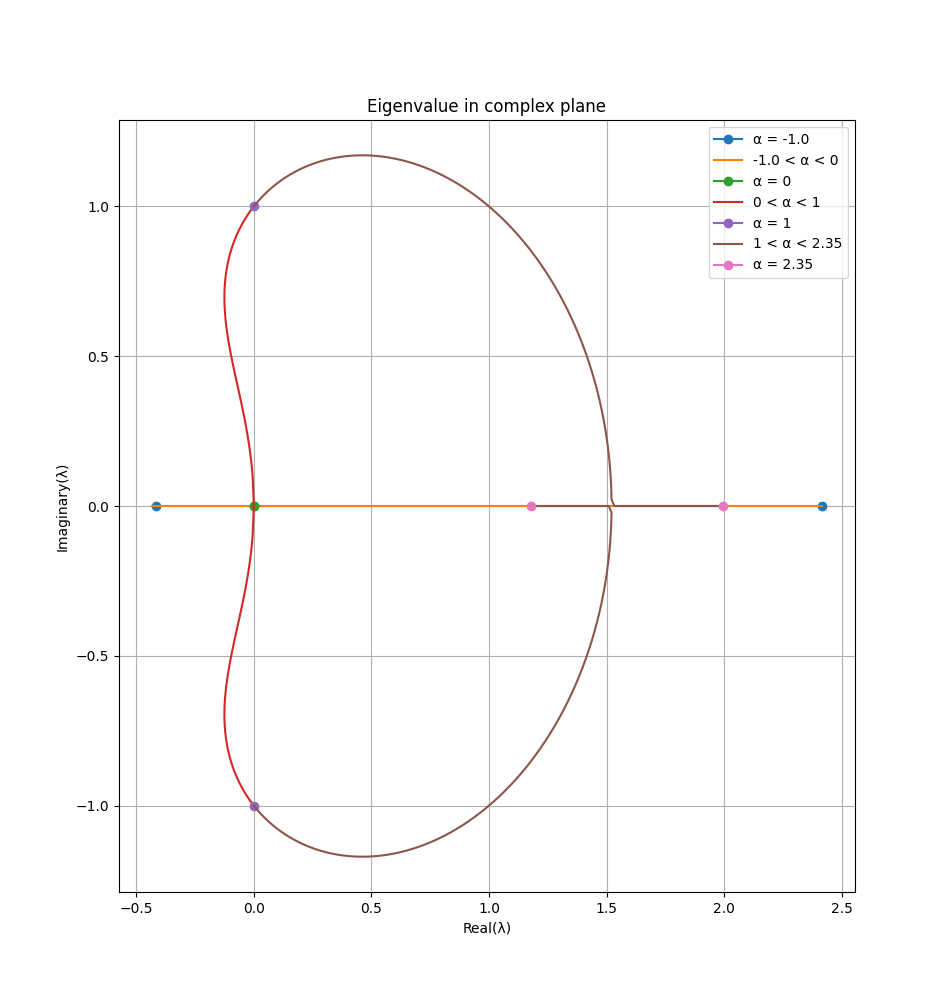
\includegraphics[width=0.8\linewidth]{eigenvalues.png}
    \captionof{figure}{Eigenvalues on complex plane}
    \label{fig:1}
\end{center}

\section{Appendix}

The proof of Theorem \ref{thm:1} is given below.

\begin{proof}
    Define the elements of matrix $A\in\R^{2\times 2}$ as
    \begin{equation}
        A = \mat{a & b \\ c & d}
    \end{equation}
    with $a,b,c,d\in\R$. Then, $A$'s characteristic equation is
    given by:
    \begin{align*}
        (a - \lambda)(d-\lambda) - bc 
            &= \lambda^2 - (a + d)\lambda + (ad - bc) \\
            &= \lambda^2 - \Tr \lambda + \Det \\
            &= 0
    \end{align*}
    So by the quadratic formula, the eigenvalues $\lambda_1,\lambda_2\in\C$
    of $A$ are given by
    \begin{equation}
        \lambda_{1,2} = \frac{1}{2}\biggl(
            \Tr \pm r
        \biggr)
    \end{equation}
    where $r\in\C$ is given by $r = \sqrt{\Tr^2 - 4\Det}$.
    ($\lambda_1$ corresponds to (+) and $\lambda_2$ to (-) of the ($\pm$).)

    We check the sign of each of $\Re(\lambda_{1,2})$   
    to determine stability based on the eigenvalue characterization
    given in class.
    Note that $\Re(r) \geq 0$ because of the square root
    (where $\Re$ denotes the real component!).  We also note that 
    $r$ is related to $|\Tr|$ based on the sign of $\Det$. For $\Det < 0$
    we have
    \begin{equation*}
        r = \sqrt{\Tr^2 - 4\Det} > \sqrt{\Tr^2} = |\Tr|,
    \end{equation*}
    for $\Det = 0$,
    \begin{equation*}
        r = |\Tr|,
    \end{equation*}
    and for $\Det > 0$,
    \begin{equation*}
        r < |\Tr|.
    \end{equation*}
    The stability for each set of conditions
    given in the theorem follows.


    \begin{letterenum}
        \item For $\Tr > 0$, we have
        \begin{equation}
            2\Re(\lambda_1) = \Re(\Tr + r) > 0
        \end{equation}
        so the system is unstable. (We will just check $\Re(\Tr \pm r)$ and omit the
        2$\Re(\lambda_{1,2})$ going forward when convenient.)
        For $\Det > 0$, we have $r > |\Tr|$ so that
        \begin{equation}
            \Re(\Tr + r) > \Re(\Tr + |\Tr|) \geq 0
        \end{equation}
        so again the system is unstable. For $\Tr = \Det = 0$, we have
        $\lambda_{1,2} = 0$ so a jordan block of with eigenvalue 0 and dimension
        2 $\Rightarrow$ unstable. So (a) holds.
        \item If $\Tr < 0$ and $\Det = 0$, then $r = -\Tr$ and
        \begin{equation}
            \lambda_1 = \Tr + r = 0 \qquad \lambda_2 = 2\Tr < 0
        \end{equation}
        so the system is (internally) stable. For $\Tr = 0$, $\Det > 0$,
        \begin{equation}
            \lambda_{1,2} = 0 \pm 2i\sqrt{\Det}
        \end{equation}
        and while $\Re(\lambda_1) = \Re(\lambda_2) = 0$, since the imaginary
        component is nonzero, $\lambda_1 \neq \lambda_2$ and each jordan
        block has dimension 1. Therefore, the system is again stable and (b)
        holds.

        \item For $\Tr < 0$ and $\Det > 0$, we consider first the case
            where $\Tr^2 - 4\Det < 0$. Then $\Re(r) = 0 \Rightarrow$
            $\Re(\lambda_{1,2}) = \Tr < 0 \Rightarrow$ the system is
            exponentially stable.

            Otherwise, $r$ is real and $0 \leq r < |\Tr|$ so that
            \begin{equation}
                \Re(\Tr - r) \leq \Re{\Tr + r} < \Tr - \Tr = 0.
            \end{equation}
            So again the system is exponentially stable.
    \end{letterenum}



\end{proof}

\end{document}
